\chapter{Formalism}\label{chap:Formalism}

This chapter introduces the reader to the more rigorous concepts and mathematical background that will required to fully understand the material presented in the later chapters of this dissertation. 

A discussion of multiplexing and signal-to-noise ratio will be discussed, as well are various coding schemes used in various notable computational sensors as well as the ones in this disseration. 


The vast majority of modern optical sensing involves an \acrfull{adc} step, which creates discrete digital values from a physical phenomena. Therefore, we will concentrate on continuous-to-discrete and discrete-to-discrete measurements. This not only makes the formalism we will discuss more relavent but in many cases it will simplify the mathematics. 

As described earlier in \Cref{chap:Introduction}, a \gls{measurement} is a map from the physical signal-of-interest \gls{objvec} to the measurement data \gls{measvec}. The solutions to the electromagnetic wave equation are linear in free space so the propagation of electromagnetic radiation is linear. We can also approximately model the response of our sensors as linear. Thus we can write the measurement as an integral
%
\begin{equation}
	g_m = \int \mb{f}( \mb{x} ) h_m ( \mb{x} ) d \mb{x}
\end{equation}
%
where $ h_m ( \mb{x} ) $ is the continuous-to-discrete measurement process from point $ \mb{x} $ to discrete measurement index \gls{m}. We can write the continuous signal-of-interest as a superposition over a basis 
%
\begin{equation}
	f( \mb{x} ) = \sum_{n} f_n \psi_n ( \mb{x} )
\end{equation}
%
This allows us to express the measurement of any optical phenomena as a matrix multiplication
%
\begin{equation}
\mathbf{g} = \mathbf{Hf}
\label{eq:gHf}
\end{equation}
%
where \gls{measvec} is now a measurement data vector and \gls{objvec} is the discrete representation of the object signal-of-interest and $\mb{H}$ is the matrix which describes measurement process. For brevity we will refer to the \gls{objvec} as the object and $\mb{H}$ as either the sensing matrix or the measurement matrix. \Cref{eq:gHf} represents the forward model in a wide variety of computational sensors. The object \gls{objvec} is a vector in \gls{n} dimensional vector space and the measurement \gls{measvec} is a vector in \gls{m} dimensional vector space. In general $m \neq n$. Note that \Cref{eq:gHf} is an extremely useful way to represent the forward model in optics, since it allows us invoke a vast amount of computationally attractive numerical techniques which are dedicated to linear systems.

In the real-world noise degrades the measurements 
\begin{equation}
	\mb{g}=\mb{Hf} + \mb{e}	
\end{equation}
where \gls{noisevec} is additive noise. Additive noise is noise which is independent of the signal. An example of additive noise includes the thermal noise generated by the random fluctuations of the charge carriers from \gls{ccd} electronics. A different type of noise called multiplicative noise also exists, but will not be considered in this dissertation. 

\section{Isomorphic Sensing}

In an isomorphic measurement, where the goal is a one-to-one mapping of object points to measurement points, the measurement matrix is often modeled with the identity matrix
\begin{equation}
	\mb{H}=\mb{I}	
\end{equation}


We can get an idea of how much error exists in an isomorphic measurement through invoking the weighing example again. This example was originally discussed in book \cite{harwit2012hadamard} but it is so useful in the context of this dissertation I will briefly summarize it here. In the weighing example, let's say we have $4$ objects with true unknown weights $f_{1}, f_{2}, \cdots, f_{4}$. We record the measured weights $g_{1}, g_{2}, \cdots, g_{4}$ with additive noise (random error)  $ e_1, e_2, \cdots, e_4 $. The forward model with noise is 
\begin{equation}
	\left[ \begin{matrix} g_1\\ g_2\\ g_3\\ g_4\end{matrix} \right] = \left[ \begin{matrix} 1& 0& 0& 0\\ 0& 1& 0& 0\\ 0& 0& 1& 0\\ 0& 0& 0& 1\end{matrix} \right] \left[ \begin{matrix} f_1\\ f_2\\ f_3\\ f_4\end{matrix} \right] + \left[ \begin{matrix} e_1\\ e_2\\ e_3\\ e_4\end{matrix} \right] 
	\label{eq:gHfpluse}
\end{equation}
The estimated weights \gls{estobjvec} are the measurements  $ \mathbf{g} $
\begin{equation}
	\mathbf{ \hat{ f }} = \mathbf{g} 
\end{equation}
Where the error between the estimated weights and the actual weights is the error $ \mb{n} = \mbh{f} - \mb{f} $. For our purposes the assumption of a zero mean distributed noise is a good assumption. This allows us to assume the the isomorphic measurements are unbiased. For an unbiased estimator, the mean squared error of the estimated weight is the variance
\begin{equation}
	E [ ( \mb{e} )^2 ] = E [ ( \mbh{f} - \mb{f} )^2 ] = \sigma^2.
\end{equation}
The smallest possible mean square error is limited to the variance of the noise. Now, I will show how multiplexing codes can be used to reduce the mean square error of the estimate. 

\section{Multiplexing}

As we discussed in \cref{chap:Introduction}, \gls{multiplexing} is an extremely useful technique for overcoming trade-offs in traditional optical sensing. Now it is time to discuss and demonstrate the quantitative advantages provided by multiplexing. 

In a multiplexed measurement, each element in the measurement vector \gls{measvec} is a weighted linear combination of the elements in the object vector. Therefore the measurement matrix $\mb{H}$ is no longer an identity matrix. 



\subsection{Coding Schemes}\label{subsec:codingschemes}

We will now discuss formally the properties, advantages and disadvantages of several popular multiplex coding schemes used in computational sensing especially in dispersive spectroscopy such as the Hadamard, S-Matrices, and random coding. 

A Hadamard matrix of order $n$ is defined as a matrix \gls{hadamardn} as the $n \times n$ matrix whose elements consist of $+1$'s and $-1$'s and satisfies the following property:
\begin{equation}
	\mb{H}_{n}^T \mb{H}_{n} = \mb{H}_{n} \mb{H}_{n}^T = n I_{n}
\end{equation}
where $\mb{I}_n$ is an $n \times n$ indentity matrix. 

In multiplex spectroscopy and imaging, Hadamard codes are extremely popular for a variety of reasons. Hadamard codes are provably optimal in the case where we are allowed to take a full set of measurements, meaning that \gls{objvec} and \gls{measvec} from \cref{eq:gHf} are both vectors in $n$ dimensional space and when one uses both $+1$'s and $-1$'s in the code \cite{harwit2012hadamard}.  In this case, Hadamard codes achieves the minimal the mean square error defined as
\begin{equation}
	\text{MSE} = \frac{1}{n} ( e_1 + e_2 + \cdots e_n )^2 
\end{equation}

In the weighing example, we can get negative measurements by using a balancing scale instead of a spring scale. An Hadamard multiplexed measurement would look like
\begin{equation}
\left[ \begin{matrix} g_{1}\\ g_{2}\\ g_{3}\\ g_{4}\end{matrix} \right] =\left[ \begin{matrix} +1 +1 +1 +1 \\ +1 -1 +1 +1 \\ +1 -1 -1 +1 \\ +1 -1 -1 +1 \end{matrix} \right] \left[ \begin{matrix} f_{1}\\ f_{2}\\ f_{3}\\ f_{4}\end{matrix} \right]
\end{equation}
This means that in the first measurement all 4 items at placed in the same pan. In the second measurement items 1 and 3 are in the same pan while items 2 and 4 are in the opposite pan, etc \cite{harwit2012hadamard}. We have four equations and four unknowns so we can solve for the estimates using algebra

\begin{align*}
  \hat{f}_1 &= \frac{1}{4} (g_1 + g2 + g2 +g4) \\
  &= f_1 + \frac{1}{4}(e_1 + e2 + e3 + e4) \\
        \mathrel{\makebox[\widthof{=}]{\vdots}} \\
  \hat{f}_4 &= \frac{1}{4} (g_1 - g2 - g2 +g4) \\
  &= f_4 + \frac{1}{4}(e_1 - e2 - e3 + e4)
\end{align*}
The mean square error of the $m^{th}$ measurement  
\begin{equation}
	E [ ( \hat{f}_{m} - {f}_{m} )^2 ] = \frac{1}{4} \sigma^2.
\end{equation}
which is $4$ times lower than using an isomorphic measurement scheme. In general, the \gls{mse} of a Hadamard measurement is 
\begin{equation}
	\text{MSE} = \frac{\sigma^2}{N_{\lambda}}
	\label{eq:hadamardmse}
\end{equation}
where \gls{numspecchan} is the number of spectral channels, which is equal to the number of measurements \gls{nummeas}. Hotelling proved in 1944 that for a measurement matrix with elements $h_{mn} \in [-1, +1]$ the lowest possible MSE for the case of a full set of measurements is with a linear unbiased estimator is $\text{MSE} = \frac{\sigma^2}{N_m}$ \cite{brady2009optical}. So, one cannot possibly do better than Hadamard coding in this case. We will see later in other special cases that we can beat Hadamard codes.

In many practical cases in computational sensing, making a code with simultaneous positive and negative modulation of the signal is not possible. For incoherent light, the response is linear in intensity. In the case where one has the ability to make a full set of measurements but is limited to elements of $+1$'s and $0$'s, an S-Matrix code minimizes the \gls{mse} \cite{harwit2012hadamard}.

In the weighing example, a spring balance rather than a two pan scale analogous to this situations. 
\begin{equation}
\left[ \begin{matrix} g_{1}\\ g_{2}\\ g_{3}\\ g_{4}\end{matrix} \right] = 
\left[ \begin{matrix} 0 & +1 & +1 & +1 \\ +1 & +1 & 0 & 0 \\ +1 & 0 & +1 & 0 \\ +1 & 0 & 0 & +1 \end{matrix} \right]
\left[ \begin{matrix} f_{1}\\ f_{2}\\ f_{3}\\ f_{4}\end{matrix} \right]
\end{equation}
So items 2, 3, and 4 are weighed together, then 1 and 2, and so on. Solving the system of equations in a silimar fashion as before in the Hadamard weighing example we find that the mean square error for the $m^{th}$ measurement when weighing 4 items is 
\begin{equation}
\text{MSE} = E [ ( \hat{f}_{m} - {f}_{m} )^2 ] = \frac{7}{9} \sigma^2.
\end{equation}
Which reduced the \gls{mse} compared to the isomorophic measurement scheme but it is less of a reduction compared to the Hadamard measurement scheme. The \gls{mse} of the S-Matrix is approximately a factor of 4 increase compared to the Hadamard matrix coding scheme. 

In the case when the full set of measurements are availible, random coding schemes are provably sub-optimal to compared to Hadamard and S-Matrix codes. However, they should not be ignored because in compressive sensing, certain theoretical garuntees exist for random coding that do not exist for Hadamard and S-Matrix codes. Sometimes, the physics of the situation forces a random coding scheme. There is little literature on the performance of random coding schemes. At the time of this writing (2016), I am unaware of an optimality proofs for random codes when one has a full set of measurements availible. 

\subsection{The Fellgett Advantage}

The \gls{Fellgett advantage} is the improvement in \gls{snr} that occurs when an instrument takes multiplexed measurements compared to isomorphic measurements \cite{fellgett1958principes, davis2001fourier}. Physically the \gls{Fellgett advantage}  occurs because a single detector element produces a noise contribution whether it's sampling a single part of the object or multiple parts of the object. Maximizing the \acrfull{snr} of the estimated object signal-of-interest for a given system throughput and detector noise is major design consideration in computational optical sensing particularly in the area of spectroscopy. In spectroscopy, there are two well known multiplex schemes, the Hadamard multiplexing in dispersive spectrometers and the interferometric spectrometer . 

The \gls{fts} architecture is a similar to the Michelson interferometer, see Figure \ref{fig:fourierTransformSpec}.The \gls{fts} operates by taking the autocorrelation of the complex electric field as a function of time delay by moving one of the mirrors in the interferometer \cite{davis2001fourier}. The Wiener-Khinchin theorem says that for a wide-sense stationary random process, the Fourier transform of the autocorrelation is the power spectral density. Thus a computational post-processing step is required to reconstruct the spectrum from the measurement data. Since the \gls{fts} measures combinations of multiple wavelengths at each detector readout it also exhibits the \gls{Fellgett advantage}.

The advantage that multiplexing provides over an isomorphic measurement depends on the coding sceheme. We've just seen that for a Hadamard coding scheme the \gls{mse} is given by \Cref{eq:hadamardmse}. It turns out that for a \gls{fts} the \gls{mse} obtained is a factor of two greater than the Hadamard multiplexing scheme \cite{tai1976fourier}. 

\begin{equation}
	\text{MSE} = 2 \frac{\sigma^2}{N_{\lambda}} 
\end{equation}

\begin{figure}
    \centering
    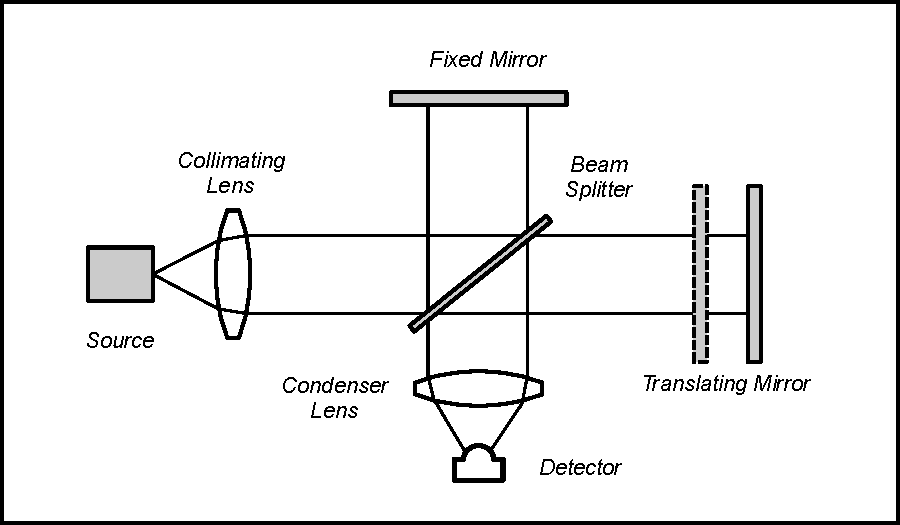
\includegraphics[scale=1]{fourierTransformSpec}
    \caption{The architecture of the Fourier Transform Spectrometer.}
    \label{fig:fourierTransformSpec}
\end{figure}

\section{Principal Component Analysis}

Principal component analysis (PCA) is a technique that attempts to recast a dataset in manner which allows us to maximally discriminate the data with just a few vectors. The first vector points in the direction of maximum variance. The second vector points in a direction that also maximizes variance but is orthogonal to the first vector and so on. These new vectors are called the \emph{principal components}. We will say the \emph{rows} of matrix $\mb{P}$ are the principal components. 

Let's say we have a dataset $\mb{S}$ which consists of $N$ spectra with \gls{numspecchan} spectral channels. Instead of looking at the data as just intensity versus spectral channel, \gls{pca} attempts to construct a set of new vectors (also called features) that show as much variation in the spectra as possible. In other words, first direction (principal component) is used to recast the data to look as different (uncorrelated) as possible. This allows us to discriminate the data, as best we can with just one direction. The second principal component is the direction that provides the second most ability to discriminate the data, and so on. 

The covariance matrix is defined as
\begin{equation}
\mb{C_{X}} = \frac{1}{N} \mb{S} \mb{S}^{T}.
\end{equation}
Each element in the covariance matrix $C_{Xmn}$ is the covariance of the $m^{th}$ spectrum $\mb{s}_m$ and the $n^{th}$ spectrum $\mb{s}_n$. 
\begin{equation}
C_{Xmn} = \frac{1}{N} \mb{s}_m \mb{s}_n^{T}.
\end{equation}

Note that large covariance means they look quite alike and therefore are difficult to disambiguate.

If the entire collection of spectra $\mb{S}$ were mutually orthogonal, being able to tell one spectrum apart from another would be easy. You would just have a collection of spikes at different spectral channels. The covariance matrix in this case would be a diagonal matrix. 

Since there is typically some redundancy between spectra, the off-diagonal elements of the covariance matrix will be non-zero. The principal components allow us to recast the data to make it as uncorrelated as possible in a new basis. 
\begin{equation}
	\mb{Y} = \mb{PX}
\end{equation}
where $\mb{Y}$ is the data projected onto the principal component basis $\mb{P}$. The covariance of the projected data
\begin{equation}
	\mb{C_{Y}} = \frac{1}{N} \mb{Y} \mb{Y}^{T} 
\end{equation}
is a now diagonal matrix. Indeed, the principal components are the optimal way to discriminate the spectra in the dataset \cite{}.

It turns out there is a way to calculate the principal components in closed form. The \emph{eigenvectors of the covariance matrix are the principal components} \cite{shlens2014tutorial}. 

Since the full set of principal components forms a basis, each spectra $\mb{s}$ in $\mb{S}$ can be written as a superposition of principal components without any error
\begin{equation}
\mb{s} = \sum_{\lambda = 1}^{N_{\lambda}} y_{\lambda} \mb{v}_{\lambda}
\end{equation}
In many cases, only a few of the first principal components are needed in the summation to approximate the original data well.
\begin{equation}
{\mb{s}} \approx \sum_{\lambda = 1}^{M} y_{\lambda} \mb{v}_{\lambda}
\end{equation}
Where $M \ll N_{\lambda} $. Note that each eigenvector has an associated eigenvalue. The eigenvalues are also informative because they can tell us how many principal components are really needed to discriminate all of the spectra. The magnitude of the eigenvalue tells us how well it's associated eigenvector is at discriminating the data.

This is another reason why \gls{pca} is so useful. It can be used as a type of lossy compression code and as a measurement matrix for compressive sensing. Simply project the data onto the first several principal compoenents associated with the largest $M$ eigenvalues. 

The \gls{afssi-c} relies on a variation of Principal Component Analysis (PCA) for discriminating between spectra. In addition to \gls{pca} the AFSSI-C uses a Bayesian probability to create adaptive codes. We will now discuss some of fundamentals of Bayesian probability and the Log-likelihood ratios. 

\section{Bayesian Rules and Log-Likelihood Ratios}

\section{Compressive Sensing}



\subsection{The Nyquist-Shannon Sampling Theorem}

The Nyquist-Shannon Sampling Theorem states one must sample a signal with a sampling rate that is at least twice the maximum frequency of the signal to prevent aliasing \cite{shannon1949communication}.



\begin{equation}
	g_{mn} = \int\displaylimits_{\infty}^{\infty} \int\displaylimits_{\infty}^{\infty}   \int\displaylimits_{-X/2}^{X/2} \int\displaylimits_{-Y/2}^{Y/2} \mb{f}( \mb{x} ) h_i ( \mb{x} ) d \mb{x}
\end{equation}

In a linear shift-invariant imaging system, the continuous object is blurred by the shift-invariant \gls{psf} . The image is sampled  

optical imaging system with a \gls{fpa} this reduces to

\begin{equation}
	g_{mn} = \int\displaylimits_{\infty}^{\infty} \int\displaylimits_{\infty}^{\infty}   \int\displaylimits_{-X/2}^{X/2} \int\displaylimits_{-Y/2}^{Y/2} \mb{f}( \mb{x} ) h_i ( \mb{x} ) d \mb{x}
\end{equation}


\subsection{Sparsity, Incoherence, and the Restricted Isometry Property}

At first glance, compressive sensing is unintuitive. Going back to the weighing example, if we have hundreds of itmes we can group the items together to increase the precision of our measurements. However, we still have to take as many measurements as their are items, to solve for their weight. If the number of measurements is less than the number of objects, then a unique solution is impossible. If we have some sort of helpful information, we can significantly reduce the number of solutions, discarding away solutions that are inconsistent with this prior information. 

In compressive sensing, this helpful knowledge is called \emph{sparsity}. A signal is sparse if only a few elements of the signal is non-zero. For compressive sensing to work, the signal-of-interst itself doesn't need to be sparse.  if one only needs to describe it with a few representation vectors relative to the native dimensionality of the signal. Note that the sign  Sparsity is quite similar to how compressiable a signal is. Most real world signals aren't sparse, they are compressible. However, we know from lossy compression techinques that we can throw away most of the data, that much of the information is not sparse. The reconstruction algorithms rely on the assumption of sparsity to correctly estimate the original signal from the small number of measurements \cite{}.

The actual question of how to code the analog signal-of-interest to produce the most compressive measurements as possible is still an active area of research \cite{}. Many in the compressive sensing community refer to the codes as the measurement basis. This interpretation of the coding scheme allows us to think of the measurement data as projections of the signal-of-interst onto a set of vectors. Incoherence is the concept that the measurement basis and the represetation basis should have low correlation with each other. The more incoherent---lower correlation---the two bases are, the higher the probability of succesful reconstruction of compressive measurements. Random matrices have a high probability of being incoherent with any basis \cite{candes2008introduction}, which is why they are so popular in experimental prototypes \cite{} since it simplified the task of having to design the measurement basis. However, as we will see random measurements do not always lead to the best reconstruction results since they are agnostic to the signal-of-interest. The choice of the measurement basis can be a difficult task depending on the application, however it has 

oherence,  However, mathematicians have shown that the measurement basis should have a low maximum correlation with the representation basis, the basis in which the object signal has a sparse representation. This allows the signal to get 


scheme relies of the coherence of the representation basis and the measurement basis. Up till now the representation basis has been the canoncial Dirac basis. 

Quite surpriseling, Other than sparsity, when other knowledge of the signal can be made often random measurements are the optimal measurements. 



\subsection{Inversion}

\subsubsection{Least Squares}

Suppose 

\begin{equation}\label{eq:lineareq1}
	\mb{g} = \mb{Hr} 
\end{equation}

Given \smb{g} and \smb{H} we want to solve for \smb{r}. If the matrix is full rank then we can simply multiply both sides of equation \ref{eq:lineareq1} by $\mbi{H}$ 

\begin{equation}
	\mbi{H} \mb{g} = \mbi{H} \mb{Hr} = \mb{I} \mb{r} = \mb{r}
\end{equation}

If \smb{H} is not full rank then its inverse does not exist. However we can try to find a solution \smbh{r} that minimizes the least squared error. This is called the \emph{Least Squares Solution} also known as the \emph{Least Squares Estimator}, \emph{Ordinary Least Squares} and by many other names. We define the squared error as

\begin{equation}\label{eq:squarederror1}
	\mathbf{ \lVert \mathbf{e} \rVert }^2 =    \mb{ \lVert \mb{Hr-g} \rVert }^2
\end{equation}

\noindent To minimize the error, we take the derivative of equation \ref{eq:squarederror1} with respect to \smb{r} and set it equal to zero and solve for \smb{r}. The full derivation which shows each step is given in Appendix \ref{app:Derivation of the Least Squares Estimator}. The least squares estimate:

\begin{equation}
	\hat{ \mb{r} } = ( \mbt{H} \mb{H} )^{-1} \mbt{H} \mb{g}
\end{equation}

\subsubsection{L0 and L1 Norm Minimization}

\subsubsection{LASSO and sparsity regularization}

$  \mathfrak{F} \{ \iint\limits_{a}^{b}  g( \xi, \eta )  h( x - \xi, y - \eta )  d \xi d \eta \}  $

%\bibliographystyle{IEEEtranS}  
%\bibliography{ThesisBib}



